\chapter{Firmware}
\label{Firmware}
% ================ Einstellungen =======================
\thispagestyle{fancy} \rhead{\slshape Firmware}
% ======================================================
Die Firmware wurde auf einen ATMega 328p Mikrochip geflashed (siehe Abbildung \ref{fig:ATMega328p}). Für die Kommunikation (UART) mit dem Bluetoothmodul ist eine zusätzliche Softwareserial (Pins PD2 \& PD3) zur üblichen seriellen Schnittstelle (Pins PD0 \& PD1) implementiert, da der ATMega 328p nur ein UART Interface (TXD \& RXD) auf den Pins PD0 \& PD1 hat. Der ATMega 328p wird mittels einem ISP (AVR-Dragon) über den sechs poligen ICSP-Header (Anhang: Schema Sheet: 3/3) JP1 geflashed.\\
Folgende Einstellungen wurden im Device Programming unter Fuses im AtmelStudio dafür vorgenommen:
\begin{itemize}
\item EXTENDED.BODLEVEL: Brown-out detection disabled
\item HIGH.SPIEN: enabled
\item HIGH.BOOTZ: Boot Flash size=2048 words start address=\$3800
\item LOW.SUT\_CKSEL: Ext. Crystal Osc. 8.0- MHz; Start-up time PWRDWN/RESET: 1K CK /14 CK + 65ms
\item EXTENDED: 0xFF
\item HIGH: 0xD9
\item LOW: 0xCF
\end{itemize}
\begin{figure}[h]
\centering
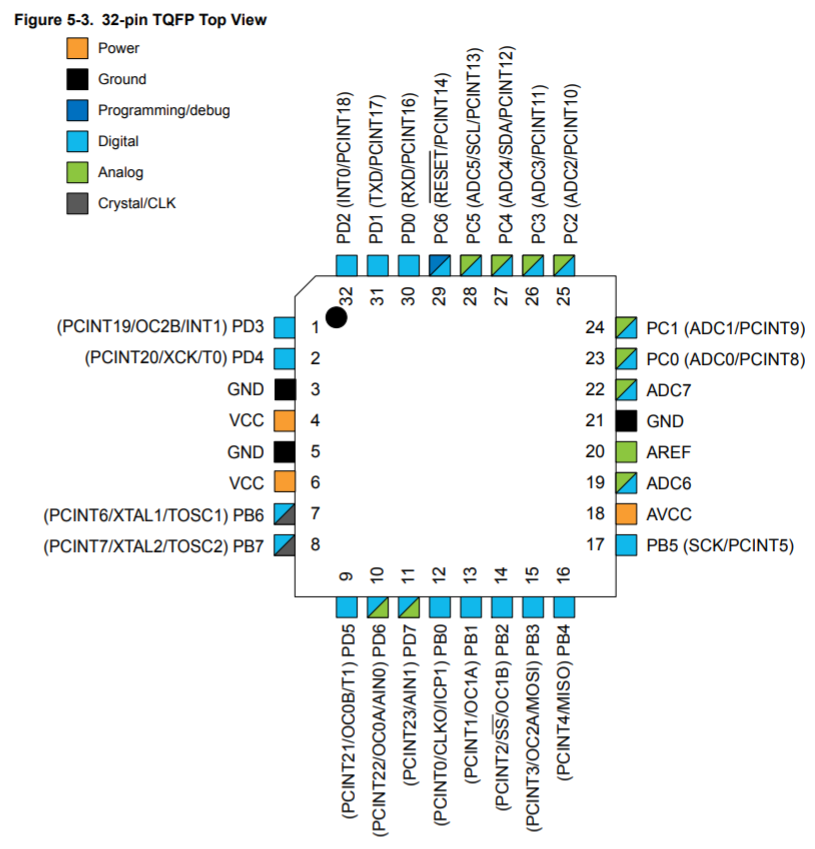
\includegraphics[width=0.59\textwidth]{Bilder/atmega328p.png} 
\caption[ATMega 328p]{ATMega 328p \cite{atmega328p}}
\label{fig:ATMega328p}
\end{figure}
\newpage
Die Firmware ist so designed, dass alle $\sharp defines$, die extern foreward declarated Funktionen und alle weiteren inkludierten Headerfiles in der Dojo.h Datei implementiert sind. Diese wird dann von der Dojo\_Functions.cpp und der Sketch.cpp Datei eingebunden. In der Abbildung \ref{fig:uml_diagramm} ist der allgemeine Aufbau der Firmware in einem UML-Diagramm visualisiert.\\
\begin{figure}[H]
\centering
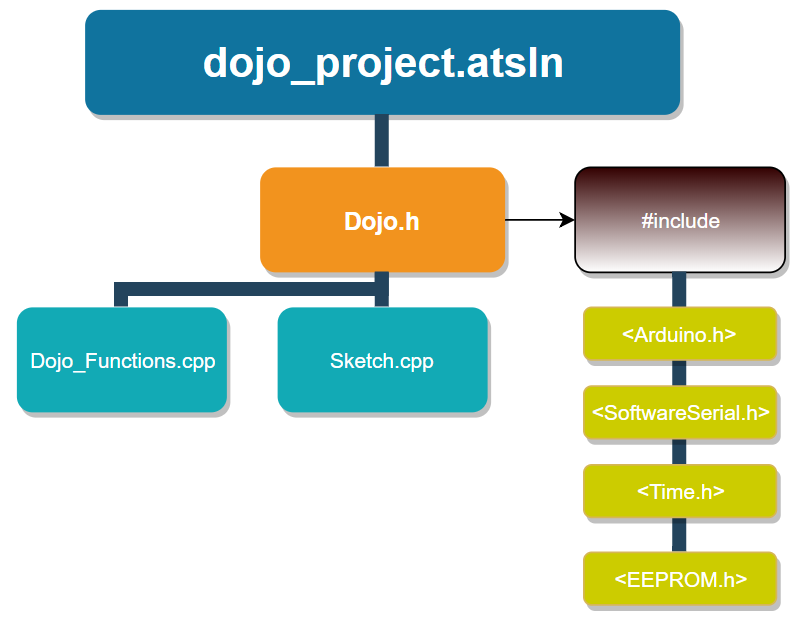
\includegraphics[width=0.8\textwidth]{Bilder/uml_diagramm.PNG} 
\caption{UML-Diagramm Firmware}
\label{fig:uml_diagramm}
\end{figure}
In der Tabelle \ref{tab:auslastung} ist die Auslastung des ATMegas mit der Endversion der geflashten Firmware dargestellt. Diese ist relativ niedrig und bietet für einen weiteren Aufbau genügend freie Memory.\\
\begin{table}[H]
\centering
\begin{tabular}{|l|r|r|}
\hline 
Program Memory Usage: & 5064 bytes & 15.5 \% Full \\ 
Data Memory Usage: & 429 bytes & 20.9 \% Full \\ 
\hline 
\end{tabular} 
\caption{Auslastung des ATMega 328p}
\label{tab:auslastung}
\end{table}
\newpage
\section{Statemachine}
Auf dem Mikrocontroller läuft eine Mealy-Statemachine mit sechs Zuständen (siehe Abbildung \ref{fig:mealy_statemachine}):\\
\begin{itemize}[leftmargin=3.2cm]
\item[INIT:] Hier wird das setup() der Firmware ausgeführt. Dabei werden alle nötigen Pinkonfigurationen initialisiert und und das WTV-Modul konfiguriert.
\item[SCAN:] Es wird vom Dojo nach IBeacons in naher Umgebung gesucht. Falls einer gefunden wurde, dann wird direkt das dazugehörige Audiofile bereitgestellt. Wird der Playbutton gedrückt, ändert sich der State zu PLAY. Ansonsten wird weiter gescanned.
\item[PLAY:] Hier werden die bereitgestellten Audiofiles abgespielt. Wird der Playbutton nochmals gedrückt, wird das Abspielen abgebrochen und der State wechselt wieder zu SCAN.
\end{itemize}
Wird das Dojo an den Computer angeschlossen, ist der Zustand des Dojos abhängig von der gewünschten Tätigkeit. Dafür wird vom Computer aus ein Befehl über das USB-Kabel gesendet, woraufhin sich der State ändert:
\begin{itemize}[leftmargin=3.2cm]
\item[GET\_LIKES:] Die vom Besucher getätigten Likes werden vom EEPROM auf den Computer transferiert.
\item[LOAD\_SD:] Sobald das Dojo in diesem State ist, schaltet der Multiplexer um und die $\mu$SD-Karte kann wie ein normaler Datenträger beschrieben werden.
\item[LOAD\_CONFIG:] Ein Ticket wird auf das interne EEPROM geladen.
\end{itemize}
\begin{figure}[h]
\centering
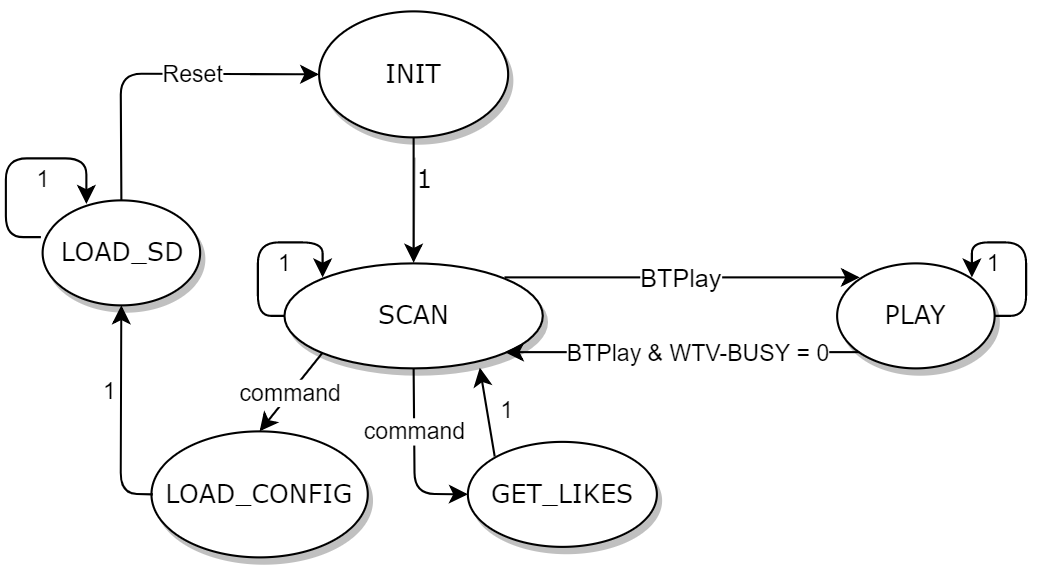
\includegraphics[width=0.9\textwidth]{Bilder/statemachine.PNG} 
\caption{Mealy-Statemachine}
\label{fig:mealy_statemachine}
\end{figure}
\newpage
 \section{Datenverwaltung}
%In diesem Kapitel wird die Datenverwaltung auf dem internen EEPROM erklärt.
Das Ticket auf dem EEPROM beinhaltet für jedes Ausstellungsobjekt zwei Bytes, das erste beinhaltet die Beacon-ID und das zweite das Zutritts- und Like-Bit.
Die ersten zwei Bytes sind reserviert und beinhalten die Anzahl gespeicherter Beacons und ein Sprachcode: 0 für die erste Sprace, 1 für die zweite.
Da auf der $\mu$SD-Karte die Dateien der zwei Sparchen abewechslungsweise und in gleicher Reihenfolge wie im EEPROM aufgelistet sind, muss nur der Index der Beaon-ID übergeben werden damit die korrekte Audiodatei abgespielt werden kann: \\
\texttt{(BeaconIndex - 2) * 2 + Sprachcode}.
\section{Validierung}
%Hier wird die Validierung der kompletten Firmware sowie dessen Ergebnisse dargelegt. 
Die Validierung der Datenverwaltung wurde mit Unittests vom PC aus gemacht. Dabei wurde ein mit Zufallszahlengenerator generiertes Ticket über die serielle Schnittstelle auf das EEPROM geschrieben und dann wieder eingelesen. Diese Validierung wurde direkt auf dem Arduino UNO Board gemacht und hat funktioniert.
\\[0.5cm]
Auf dem MCU sind am Ende noch Probleme beim Auslesen des Receivebuffer von der seriellen Schnittstelle über das USB-Kabel zum Computer aufgetaucht. Dabei konnten über mySerial.available() die vom Computer gesendeten Befehle nicht ausgelesen werden. Mit dem Oszilloskop sind die gesendeten Befehle auf dem PD0 zwar messbar, allerdings können von der Seite des MCUs aus diese \glqq Daten\grqq\; nicht detektiert werden. Deshalb funktioniert die Kommunikation vom Computer zum MCU auf dem Prototyp nicht wie geplant. Umgekehrt vom MCU zum Computer können aber Daten gesendet werden. Um die States zu ändern, wurden nun für die gesamte Funktion Taster zur Stateänderung verwendet, damit die Statemachine und der Ablauf der Firmware funktioniert.
\\[0.5cm]
Dabei sind die Tasterfunktionen:
\begin{itemize}[leftmargin=1.2cm]
\item[SW1:] Ändert den State zu LOAD\_SD
\item[SW2:] Ändert den State zu PLAY
\item[SW3:] Ändert den State zu LOAD\_CONFIG
\end{itemize}
Ein weiterer Aspekt, welcher dazu führt, dass für einen nächsten Prototyp des Dojos möglicherweise ein anderer Mikrochip benutzt wird ist, dass der ATMega 328p nur zwei external Interrupts hat (Abbilung \ref{fig:ATMega328p} Pins PD2-INT0 \& PD3-INT1). Diese sind momentan aber mit der Softwareserial belegt, weshalb mit den Taster nicht auf diese zugegriffen werden kann. Genauso gab es Konflikte mit der Softwareserial Library, die Tasterinterrupts über Pin Change Interrupts anzusteuern. Darum werden jetzt für die gesamte Funktion des Prototyps die Taster nach jedem scan() abgefragt und die Statusled zum togglen gebracht, wenn der Taster detektiert wurde.
\\[0.5cm]
Die $\mu$SD-Karte kann als normaler Datenträger mit den Audiofiles beschrieben werden. Zu beachten ist einfach, dass dies nur über einen Computer mit Linux als Betriebssystem funktioniert.